\section{Compito Due: contesto, complemento e distanza libera}
\label{sec:compito2}

Il calcolo è disponibile come metodo \code{CalcoloChiusura.calcola(griglia,
x, y)} e lavora su qualunque griglia, in particolare su quelle prodotte dal
generatore e salvate in JSON. Nell'applicazione viene invocato da \cmin{}
a ogni chiamata; la traccia osserva che \cmin{} comprende l'elaborazione
del Compito Due (pag.~34). Lo stesso calcolo è disponibile anche da solo,
dalla riga di comando (\cref{sec:applicazione-chiusura}).

Nel seguito si usano le nozioni della traccia. Un \emph{cammino libero} da
$O$ è privo di ostacoli ed è formato da mosse diagonali in un solo verso
seguite da mosse rettilinee in un solo verso (\emph{tipo~1}), o dalle stesse
mosse in ordine inverso (\emph{tipo~2}); i versi sono quelli del quadrante in
cui si trova la destinazione. Il \emph{contesto} di $O$ contiene le celle
raggiungibili con un cammino libero di tipo~1, il \emph{complemento} quelle
raggiungibili \emph{solo} con un cammino di tipo~2; la loro unione è la
\emph{chiusura}. La \emph{frontiera} è formata dalle celle della chiusura
adiacenti ad almeno una cella attraversabile esterna alla chiusura.

\subsection{Distanza libera}

La distanza libera è la lunghezza di un cammino libero, cioè del cammino
minimo in assenza di ostacoli. Posti $\Delta_x = |x_D - x_O|$,
$\Delta_y = |y_D - y_O|$, $\Delta_{\min} = \min(\Delta_x,\Delta_y)$ e
$\Delta_{\max} = \max(\Delta_x,\Delta_y)$, si calcola in tempo costante:
\begin{equation}
  \dlib(O,D) = \sqrt{2}\,\Delta_{\min} + \Delta_{\max} - \Delta_{\min}.
  \label{eq:dlib}
\end{equation}
Nessun cammino fra $O$ e $D$ può essere più corto, quindi $\dlib(O,D)$ è un
limite inferiore della lunghezza di qualunque cammino fra le due celle. Il
record \code{DistanzaLibera} conserva separatamente le due componenti del
cammino libero, il numero di mosse rettilinee $\Delta_{\max} - \Delta_{\min}$
(componente ``torre'') e il numero di mosse diagonali $\Delta_{\min}$ (componente
``alfiere''), insieme al valore reale della lunghezza.

Due scelte riguardano l'aritmetica in virgola mobile:

\begin{itemize}
  \item le lunghezze sono confrontate con una tolleranza
        $\varepsilon = 10^{-10}$, perché somme di multipli di $\sqrt{2}$
        ottenute in ordini diversi possono differire nell'ultima cifra;
  \item la lunghezza infinita, usata per una destinazione irraggiungibile, è
        rappresentata da \code{Double.POSITIVE\_INFINITY}; la somma con un
        valore infinito restituisce infinito.
\end{itemize}

\subsection{Calcolo di contesto e complemento}
\label{sec:chiusura}

Il calcolo sfrutta la forma dei cammini liberi. Si considerino le otto
semirette che partono da $O$ nelle direzioni N, S, E, W, NE, NW, SE, SW e si
fermano al primo ostacolo o al bordo della griglia; nel seguito sono chiamate
\emph{linee primarie}. Ogni cella di una linea primaria è raggiungibile con
un cammino libero di sole mosse uguali, quindi di tipo~1. Le altre celle della
chiusura si ottengono con un'unica deviazione:

\begin{itemize}
  \item un cammino di tipo~1 con entrambe le componenti percorre un tratto di
        una linea primaria diagonale e poi una linea rettilinea in uno dei
        due versi che compongono la diagonale (per NE: E oppure N);
  \item un cammino di tipo~2 percorre un tratto di una linea primaria
        rettilinea e poi una linea diagonale nel quadrante corrispondente
        (per N: NW oppure NE).
\end{itemize}

Da ogni cella di una linea primaria partono quindi due \emph{linee laterali},
anch'esse interrotte dal primo ostacolo o dal bordo
(\cref{tab:direzioni}). Le celle delle laterali che partono da una diagonale
sono nel contesto; quelle delle laterali che partono da una linea rettilinea
sono raggiungibili con un cammino di tipo~2 e vengono marcate come
complemento.

\begin{table}[H]
\centering
\small
\begin{tabular}{@{}l l l@{}}
\toprule
\textbf{Linea primaria} & \textbf{Linee laterali} & \textbf{Stato delle celle laterali} \\
\midrule
N, S, E, W     & le due diagonali del quadrante (per N: NW e NE) & \code{COMPLEMENTO} (tipo 2) \\
NE, NW, SE, SW & le due rettilinee componenti (per NE: E e N)    & \code{CONTESTO} (tipo 1) \\
\bottomrule
\end{tabular}
\caption{Direzioni percorse da \code{CalcoloChiusura} a partire da ogni linea
primaria.}
\label{tab:direzioni}
\end{table}

Una cella può essere raggiunta sia da un cammino di tipo~1 sia da uno di
tipo~2. Poiché il complemento contiene soltanto le celle raggiungibili
\emph{solo} con il tipo~2, una passata finale toglie il bit
\code{COMPLEMENTO} alle celle che hanno anche il bit \code{CONTESTO}. Il
contesto e il complemento sono così calcolati insieme, come la traccia
consente (pag.~21), in un'unica scansione delle otto direzioni
(\cref{alg:chiusura}).

Ogni passo verifica soltanto la cella di arrivo. Una mossa diagonale fra due
ostacoli che si toccano per uno spigolo è quindi ammessa, come richiesto
dalla traccia. La \cref{fig:esempio}(a) mostra il risultato su una delle
griglie del piano sperimentale e la \cref{tab:stati-esempio} gli stati che ne
risultano: le 144 celle assumono otto valori diversi, ciascuno una
combinazione dei bit della \cref{tab:statocella}.

\begin{figure}[H]
  \centering
  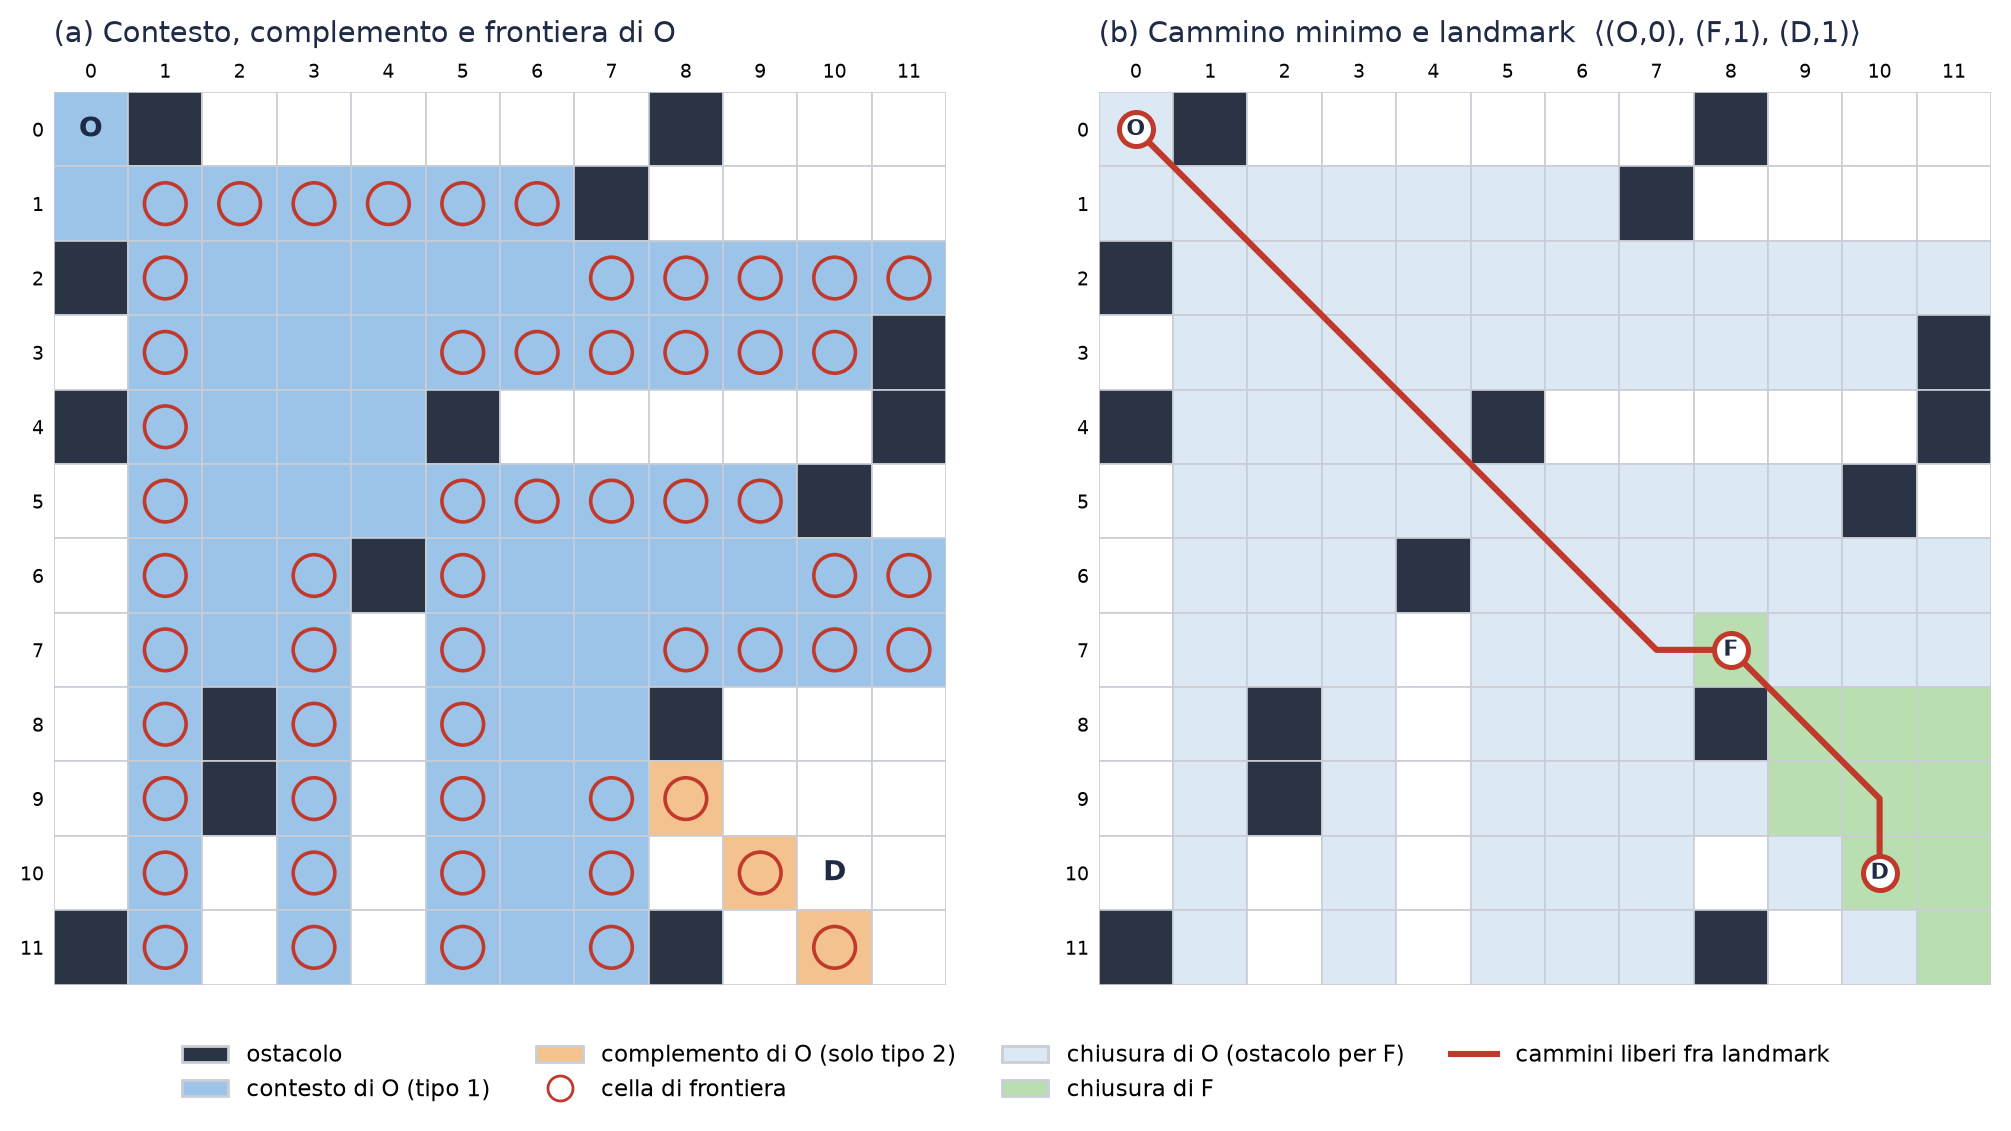
\includegraphics[width=\textwidth]{esempio_chiusura_landmark.png}
  \caption{Griglia $12\times 12$ con 15 ostacoli (seed 50), $O=(0,0)$ e
  $D=(10,10)$. (a) Contesto, complemento e frontiera di $O$ calcolati
  con l'\cref{alg:chiusura}. (b) Cammino minimo di lunghezza
  $9\sqrt{2}+2 \approx 14{,}728$ restituito da \cmin{}: $D$ non appartiene
  alla chiusura di $O$, quindi il cammino passa per la cella di frontiera
  $F=(8,7)$, la cui chiusura è calcolata trattando come ostacoli le celle
  della chiusura di $O$. I tratti fra landmark sono disegnati come cammini
  liberi a solo scopo illustrativo.}
  \label{fig:esempio}
\end{figure}

\begin{table}[H]
\centering
\small
\begin{tabular}{@{}r l l r@{}}
\toprule
\textbf{Valore} & \textbf{Bit} & \textbf{Proprietà} & \textbf{Celle} \\
\midrule
0   & \code{00000000} & libera, fuori dalla chiusura & 44 \\
1   & \code{00000001} & contesto                     & 22 \\
3   & \code{00000011} & contesto, regina             & 6 \\
5   & \code{00000101} & contesto, origine            & 1 \\
17  & \code{00010001} & contesto, frontiera          & 51 \\
19  & \code{00010011} & contesto, regina, frontiera  & 2 \\
24  & \code{00011000} & complemento, frontiera       & 3 \\
128 & \code{10000000} & ostacolo                     & 15 \\
\bottomrule
\end{tabular}
\caption{Stati delle celle nella griglia della \cref{fig:esempio}(a).}
\label{tab:stati-esempio}
\end{table}

\begin{algorithm}[H]
\caption{Calcolo di chiusura e frontiera di una cella $O$}
\label{alg:chiusura}
\begin{algorithmic}[1]
\Require griglia $g$ di dimensioni $W \times H$, cella $O$
\Ensure matrice degli stati $s$, chiusura di $O$, frontiera di $O$
\Procedure{CalcolaChiusura}{$g, O$}
  \State $s \gets$ matrice $H \times W$ con il solo bit \code{OSTACOLO} copiato da $g$
  \If{$O$ è un ostacolo} \Return $s, \emptyset, \emptyset$ \EndIf
  \ForEach{direzione primaria $d$ fra le otto}
    \ForEach{cella $c$ di \Call{Linea}{$g, O, d$}}
      \State $s[c] \gets s[c] \mathbin{|} \code{CONTESTO} \mathbin{|} \code{REGINA}$
      \State $\mathit{classe} \gets \code{CONTESTO}$ \textbf{if} $d$ è diagonale \textbf{else} $\code{COMPLEMENTO}$
      \ForEach{direzione laterale $\ell$ di $d$ (\cref{tab:direzioni})}
        \ForEach{cella $c'$ di \Call{Linea}{$g, c, \ell$}}
          \State $s[c'] \gets s[c'] \mathbin{|} \mathit{classe}$
        \EndFor
      \EndFor
    \EndFor
  \EndFor
  \ForEach{cella $c$ con $s[c]$ contenente \code{CONTESTO}}
    \State togli \code{COMPLEMENTO} da $s[c]$ \Comment{complemento esclusivo}
  \EndFor
  \State $s[O] \gets s[O] \mathbin{|} \code{ORIGINE} \mathbin{|} \code{CONTESTO}$
  \State $\mathit{chiusura} \gets \{c : s[c] \text{ contiene } \code{CONTESTO} \text{ o } \code{COMPLEMENTO}\}$
  \State $\mathit{frontiera} \gets \emptyset$
  \ForEach{$c \in \mathit{chiusura}$}
    \If{esiste un vicino $v$ di $c$ nella griglia, non ostacolo e non in $\mathit{chiusura}$}
      \State $s[c] \gets s[c] \mathbin{|} \code{FRONTIERA}$; \quad aggiungi $c$ a $\mathit{frontiera}$
    \EndIf
  \EndFor
  \State \Return $s, \mathit{chiusura}, \mathit{frontiera}$
\EndProcedure
\Statex
\Function{Linea}{$g, c, d$} \Comment{celle da $c$ (esclusa) in direzione $d$}
  \State $L \gets \seq{}$; \quad $c \gets c + d$
  \While{$c$ è nella griglia \textbf{and} $c$ non è un ostacolo}
    \State aggiungi $c$ a $L$; \quad $c \gets c + d$
  \EndWhile
  \State \Return $L$
\EndFunction
\end{algorithmic}
\end{algorithm}

\subsection{Frontiera}

Una cella della chiusura è di frontiera se almeno una delle otto celle
adiacenti è dentro la griglia, non è un ostacolo e non appartiene alla
chiusura. Le celle esterne alla griglia non contano come celle
attraversabili: se la chiusura copre tutta una griglia senza ostacoli, la
frontiera è vuota. Il tipo di una cella di frontiera si legge dal suo stato:
$t=1$ se ha il bit \code{CONTESTO}, $t=2$ altrimenti.

\subsection{Complessità}
\label{sec:complessita-chiusura}

Sia $n = WH$ il numero di celle.

\paragraph{Tempo.} La copia iniziale degli ostacoli, la passata che rende
esclusivo il complemento e la raccolta della chiusura scandiscono l'intera
griglia: $\Theta(n)$. Le linee primarie hanno lunghezza complessiva
$O(W+H)$. Le linee laterali che partono da una stessa linea primaria nella
stessa direzione sono parallele, quindi disgiunte; ogni cella può essere
attraversata al più da una laterale per ciascuna delle due linee primarie che
delimitano il suo ottante.
Le laterali visitano perciò $O(n)$ celle in totale. Il controllo della
frontiera esamina otto vicini per ogni cella della chiusura, $O(n)$.
Complessivamente il calcolo costa $\Theta(n)$, anche quando la chiusura è
piccola, perché le scansioni coprono sempre tutta la griglia.

\paragraph{Spazio.} La matrice degli stati occupa $4n$ byte (un \code{int}
per cella); la lista della chiusura e l'array della frontiera hanno al più
$n$ elementi. Lo spazio è quindi $\Theta(n)$.

Il costo lineare nella dimensione della griglia ha conseguenze sul Compito
Tre: \cmin{} calcola una chiusura a ogni chiamata ricorsiva non servita
dalla cache, quindi il suo costo è almeno proporzionale a $n$ per il numero
di chiusure calcolate (\cref{sec:analisi-teorica}).

\subsection{Applicazione}
\label{sec:applicazione-chiusura}

L'opzione \code{-{}-chiusura} esegue il solo Compito Due su una griglia
generata con i parametri della \cref{sec:compito1} oppure letta da un file
JSON prodotto dal generatore (\code{-{}-grid-input}). Per la cella $O$
indicata l'applicazione stampa la mappa della chiusura, il numero di celle di
contesto, complemento e frontiera, l'appartenenza di $D$ alla chiusura e la
distanza libera $\dlib(O,D)$, scomposta in mosse rettilinee e diagonali; con
\code{-{}-chiusura-output} salva anche gli stati di tutte le celle in JSON,
nel formato della \cref{tab:statocella}. Sulla griglia della
\cref{fig:esempio}(a) l'uscita è la seguente (le celle di frontiera
sono in maiuscolo) e i conteggi coincidono con la \cref{tab:stati-esempio}.

\begin{lstlisting}
java -jar asd-project.jar --grid-input risultati/griglie_json/scenario_02_12x12_15ost_seed50.json --origin 0,0 --destination 10,10 --chiusura
O   #   .   .   .   .   .   .   #   .   .   .
c   C   C   C   C   C   C   #   .   .   .   .
#   C   c   c   c   c   c   C   C   C   C   C
.   C   c   c   c   C   C   C   C   C   C   #
#   C   c   c   c   #   .   .   .   .   .   #
.   C   c   c   c   C   C   C   C   C   #   .
.   C   c   C   #   C   c   c   c   c   C   C
.   C   c   C   .   C   c   c   C   C   C   C
.   C   #   C   .   C   c   c   #   .   .   .
.   C   #   C   .   C   c   C   K   .   .   .
.   C   .   C   .   C   c   C   .   K   D   .
#   C   .   C   .   C   c   C   #   .   K   .
Legenda: O origine, D destinazione, # ostacolo, c contesto (tipo 1), k complemento (tipo 2), maiuscole = frontiera, . fuori dalla chiusura
Contesto: 82 celle | complemento: 3 celle | frontiera: 56 celle (53 di tipo 1, 3 di tipo 2)
O=(0,0), D=(10,10): D si trova fuori dalla chiusura di O
dlib(O,D) = 0 + 10*sqrt(2) = 14.142136 (0 mosse rettilinee, 10 diagonali)
\end{lstlisting}

\subsection{Verifica}

Oltre ai test unitari su casi costruiti a mano, \code{CalcoloChiusura} è
confrontato con un \emph{oracolo}, cioè un'implementazione di riferimento che
calcola lo stesso risultato con un metodo diverso e più semplice, così che un
errore difficilmente sia comune ai due. L'oracolo
(\code{CalcoloChiusuraOracleTest}) non usa linee primarie e laterali: per ogni
cella $c$ percorre l'unico cammino di tipo~1 e l'unico di tipo~2 da $O$ a $c$
e controlla che non attraversino ostacoli, applicando direttamente la
definizione; la frontiera è ricavata dalla chiusura così ottenuta. Il test
enumera tutte le $2^9 = 512$ disposizioni di ostacoli su una griglia
$3\times3$ e, per ogni origine libera, richiede che contesto, complemento,
chiusura e frontiera coincidano cella per cella. Un test dedicato verifica che la mossa
diagonale fra due ostacoli adiacenti per uno spigolo sia ammessa e costi
$\sqrt{2}$.
